% SparseEncoder detail (VoxelNet-style sparse conv encoder, spconv 2.x).
\documentclass[tikz,border=8pt]{standalone}
% Shared styles for the DSB architecture diagrams.
\usepackage[T1]{fontenc}
\usepackage{graphicx}
\usetikzlibrary{arrows.meta, backgrounds, calc, fit, positioning, shapes.geometric}

\definecolor{camA}{HTML}{2A78D6}
\definecolor{lidA}{HTML}{1BAF7A}
\definecolor{fusA}{HTML}{EB6834}
\definecolor{detA}{HTML}{6250D6}
\definecolor{segA}{HTML}{0E8FA8}
\definecolor{occA}{HTML}{B5482A}
\definecolor{inkA}{HTML}{262626}
\definecolor{mutA}{HTML}{6B6B6B}

\tikzset{
  blk/.style={
    draw=inkA!70, line width=0.45pt, rounded corners=2.5pt,
    align=center, font=\small, inner sep=3pt,
    minimum height=0.95cm, text=inkA, fill=white,
  },
  cam/.style={blk, fill=camA!10, draw=camA!75},
  lid/.style={blk, fill=lidA!10, draw=lidA!75},
  fus/.style={blk, fill=fusA!12, draw=fusA!80},
  det/.style={blk, fill=detA!10, draw=detA!75},
  seg/.style={blk, fill=segA!10, draw=segA!75},
  occ/.style={blk, fill=occA!10, draw=occA!75},
  io/.style={blk, fill=black!4, draw=inkA!55},
  arr/.style={-{Stealth[length=2.2mm,width=1.6mm]}, line width=0.65pt, draw=inkA!75},
  darr/.style={arr, dashed},
  tag/.style={font=\scriptsize, text=mutA},
  grp/.style={draw=mutA!70, dashed, line width=0.6pt, rounded corners=6pt, inner sep=8pt},
  hdr/.style={font=\normalsize\bfseries, text=inkA, anchor=west},
  note/.style={font=\scriptsize, text=mutA, align=left},
}


\begin{document}
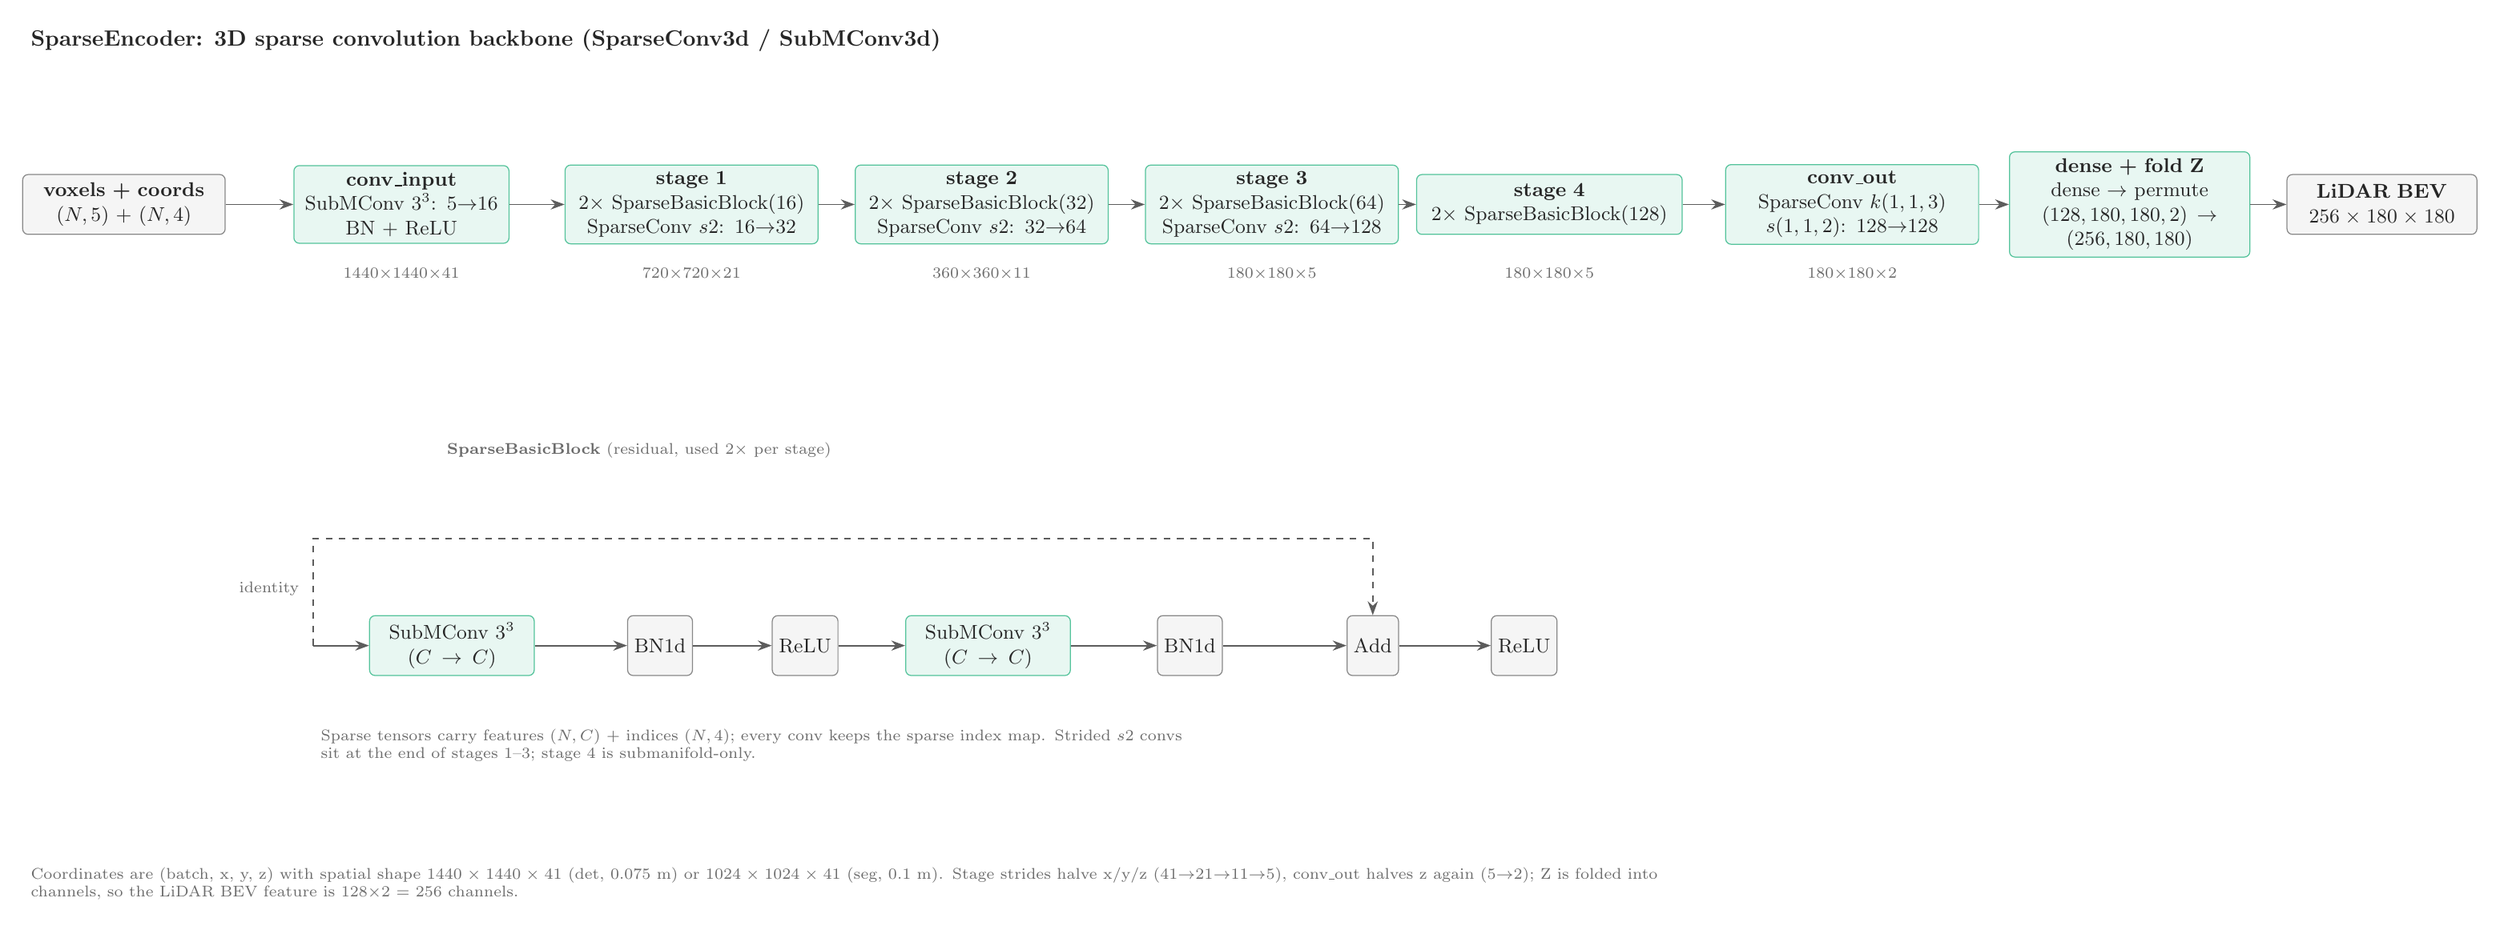
\begin{tikzpicture}

% ---------------------------------------------------------------- main chain
\node[io, text width=3.0cm] (vox) at (0,13)
  {\textbf{voxels + coords}\\$(N,5)$ + $(N,4)$};
\node[lid, text width=3.2cm] (cin) at (4.4,13)
  {\textbf{conv\_input}\\SubMConv $3^3$: 5$\to$16\\BN + ReLU};
\node[lid, text width=3.8cm] (s1) at (9.0,13)
  {\textbf{stage 1}\\2$\times$ SparseBasicBlock(16)\\
   SparseConv $s2$: 16$\to$32};
\node[lid, text width=3.8cm] (s2) at (13.6,13)
  {\textbf{stage 2}\\2$\times$ SparseBasicBlock(32)\\
   SparseConv $s2$: 32$\to$64};
\node[lid, text width=3.8cm] (s3) at (18.2,13)
  {\textbf{stage 3}\\2$\times$ SparseBasicBlock(64)\\
   SparseConv $s2$: 64$\to$128};
\node[lid, text width=4.0cm] (s4) at (22.6,13)
  {\textbf{stage 4}\\2$\times$ SparseBasicBlock(128)};
\node[lid, text width=3.8cm] (cout) at (27.4,13)
  {\textbf{conv\_out}\\SparseConv $k(1,1,3)$\\
   $s(1,1,2)$: 128$\to$128};
\node[lid, text width=3.6cm] (dense) at (31.8,13)
  {\textbf{dense + fold Z}\\dense $\to$ permute\\
   $(128,180,180,2)\to(256,180,180)$};
\node[io, text width=2.8cm] (out) at (35.8,13)
  {\textbf{LiDAR BEV}\\$256\times180\times180$};

\foreach \a/\b in {vox/cin, cin/s1, s1/s2, s2/s3, s3/s4, s4/cout, cout/dense, dense/out} {
  \draw[arr] (\a) -- (\b);
}

% resolution annotations
\node[tag] at (4.4,11.9) {1440$\times$1440$\times$41};
\node[tag] at (9.0,11.9) {720$\times$720$\times$21};
\node[tag] at (13.6,11.9) {360$\times$360$\times$11};
\node[tag] at (18.2,11.9) {180$\times$180$\times$5};
\node[tag] at (22.6,11.9) {180$\times$180$\times$5};
\node[tag] at (27.4,11.9) {180$\times$180$\times$2};

% ---------------------------------------------------------------- residual block inset
\begin{scope}[shift={(5.2,6.0)}]
  \node[tag, anchor=west] at (-0.2,3.1) {\textbf{SparseBasicBlock} (residual, used 2$\times$ per stage)};
  \node[lid, text width=2.4cm] (b1) at (0,0) {SubMConv $3^3$\\($C\to C$)};
  \node[io] (bn1) at (3.3,0) {BN1d};
  \node[io] (r1) at (5.6,0) {ReLU};
  \node[lid, text width=2.4cm] (b2) at (8.5,0) {SubMConv $3^3$\\($C\to C$)};
  \node[io] (bn2) at (11.7,0) {BN1d};
  \node[io] (add) at (14.6,0) {Add};
  \node[io] (r2) at (17.0,0) {ReLU};
  \draw[arr] (b1) -- (bn1);
  \draw[arr] (bn1) -- (r1);
  \draw[arr] (r1) -- (b2);
  \draw[arr] (b2) -- (bn2);
  \draw[arr] (bn2) -- (add);
  \draw[arr] (add) -- (r2);
  \draw[arr] (-2.2,0) -- (b1);
  \draw[arr, dashed] (-2.2,0) -- (-2.2,1.7) -| (add.north);
  \node[tag, anchor=east] at (-2.3,0.9) {identity};
  \node[note, anchor=north west, text width=14cm] at (-2.2,-1.2)
    {Sparse tensors carry features $(N,C)$ + indices $(N,4)$; every conv keeps the
     sparse index map. Strided $s2$ convs sit at the end of stages 1--3; stage 4 is
     submanifold-only.};
\end{scope}

% ---------------------------------------------------------------- notes
\node[note, anchor=north west, text width=26cm] at (-1.6,2.6)
  {Coordinates are (batch, x, y, z) with spatial shape $1440\times1440\times41$ (det, 0.075 m)
   or $1024\times1024\times41$ (seg, 0.1 m). Stage strides halve x/y/z (41$\to$21$\to$11$\to$5),
   conv\_out halves z again (5$\to$2); Z is folded into channels, so the LiDAR BEV feature is
   128$\times$2 = 256 channels.};

\node[hdr] at (-1.6,15.6) {SparseEncoder: 3D sparse convolution backbone (SparseConv3d / SubMConv3d)};

\end{tikzpicture}
\end{document}
